\section{Use Cases: Patienten- und Raumverwaltung}

Die folgenden Tabellen beschreiben die funktionalen Anforderungen an die Patienten- und Raumverwaltung, um die entsprechenden Integritätsbedingungen des Datenmodells aufzuzeigen.

% Use Case 1: Stationäre Aufnahme
\begin{table}[H]
\centering
\renewcommand{\arraystretch}{1.4}
\begin{tabular}{|p{4cm}|p{11cm}|}
\hline
\textbf{Titel} & \textbf{Stationäre Aufnahme eines Patienten und initiale Zimmerzuweisung} \\ \hline

\textbf{Kontext} & 
Sobald ein Patient stationär aufgenommen werden soll, etwa nach einer ärztlichen Einweisung oder aus der Notaufnahme heraus, wird dies durch administratives Personal initiiert.
Als Voraussetzung muss der Patient bereits im Krankenhausinformationssystem erfasst sein und aktuelle Informationen zur Zimmerbelegung müssen vorliegen, sodass eine geeignete Zuweisung erfolgen kann. \\ \hline

\textbf{Beschreibung} & 
Zur stationären Aufnahme eines Patienten wird ein bereits im System erfasster Patient einem konkreten Zimmer zugewiesen, wodurch ein aktiver Aufenthalt erzeugt wird. 
Die Zuweisung erfolgt unter Berücksichtigung der aktuellen Zimmerauslastung sowie organisatorischer Kriterien wie Station oder Fachabteilung. 
Dokumentiert wird hierbei zudem der Beginn des Aufenthalts. \\ \hline

\textbf{Besonderheiten} &
Das zugewiesene Zimmer darf noch nicht vollständig belegt sein, eine Überschreitung der Kapazität ist dementsprechend nicht möglich.\\ \hline

\end{tabular}
\caption{Use Case: Stationäre Aufnahme eines Patienten}
\end{table}

% Use Case 2: Patientenverlegung
\begin{table}[H]
\centering
\renewcommand{\arraystretch}{1.4}
\begin{tabular}{|p{4cm}|p{11cm}|}
\hline
\textbf{Titel} & \textbf{Interne Verlegung eines Patienten} \\ \hline

\textbf{Kontext} & 
Eine Änderung der aktuellen Zimmerbelegung kann beispielsweise durch medizinische Anforderungen, organisatorische Umstrukturierungen oder eine optimierte Auslastung der Stationen erforderlich sein.
Voraussetzung für eine solche interne Verlegung ist ein bereits bestehender stationärer Aufenthalt des Patienten sowie die Verfügbarkeit eines geeigneten Zielzimmers. \\ \hline

\textbf{Beschreibung} & 
Der Patient wird aus seinem aktuell zugewiesenen Zimmer in ein anderes Zimmer innerhalb des Krankenhauses verlegt.  \\ \hline

\textbf{Besonderheiten} & 
Der bestehende Buchungseintrag wird zur besseren Nachvollziehbarkeit mit dem entsprechenden Zeitstempel geschlossen und ein neuer Eintrag angelegt. 
Zudem gelten weiterhin die Beschränkungen der Kapazität auch für das neu zugewiesene Zimmer.\\ \hline

\end{tabular}
\caption{Use Case: Zimmerverlegung}
\end{table}

% Use Case 3: Patientenentlassung
\begin{table}[H]
\centering
\renewcommand{\arraystretch}{1.4}
\begin{tabular}{|p{4cm}|p{11cm}|}
\hline
\textbf{Titel} & \textbf{Entlassung eines Patienten aus dem stationären Aufenthalt} \\ \hline

\textbf{Kontext} & 
Der Use Case wird durch medizinisches oder administratives Personal ausgelöst, sobald ein stationärer Behandlungsaufenthalt abgeschlossen ist. 
Voraussetzung ist ein aktuell aktiver Aufenthalt des Patienten, der noch keinem Endzeitpunkt zugeordnet ist. \\ \hline

\textbf{Beschreibung} & 
Der aktive stationäre Aufenthalt des Patienten wird beendet, indem der zugehörige Buchungseintrag abgeschlossen wird und die Entlassung mit dem entsprechenden Zeitstempel dokumentiert wird.
Das zuvor belegte Zimmer wird dadurch wieder für zukünftige Patienten frei. \\ \hline

\end{tabular}
\caption{Use Case: Entlassung eines Patienten}
\end{table}

%TODO dann unten Teil vom Klassendiagramm einfügen
\subsection*{Resultierende Entitäten}

Aus den beschriebenen Anwendungsfällen lassen sich die notwendigen Entitäten und deren Beziehungen ableiten, wie sie im vorliegenden Datenbankschema implementiert wurden:

\begin{itemize}
    \item \textbf{Department (Abteilung):} Bildet die oberste organisatorische Einheit und gruppiert medizinische Kompetenzen sowie die zugehörigen Stationen.
    \item \textbf{Station:} Repräsentiert eine Pflegeeinheit, die funktional fest einem \texttt{department} zugeordnet ist.
    \item \textbf{Rooms (Zimmer):} Jedes Zimmer ist über die \texttt{station\_id} eindeutig lokalisierbar und einer Station zugeordnet.
    \item \textbf{Patient:} Die zentrale Entität für alle medizinischen und administrativen Prozesse, verknüpft mit den Stammdaten der Relation \texttt{person}.
    \item \textbf{Bookings (Buchungen):} Fungiert als Auflösung der Relation \textit{Patient - Room}: Sie speichert die zeitliche Dimension (\texttt{from}/\texttt{until}) der Raumbelegung und verknüpft Patienten mit ihren jeweiligen Aufenthaltsorten.
\end{itemize}

\begin{figure}[h]
    \centering
    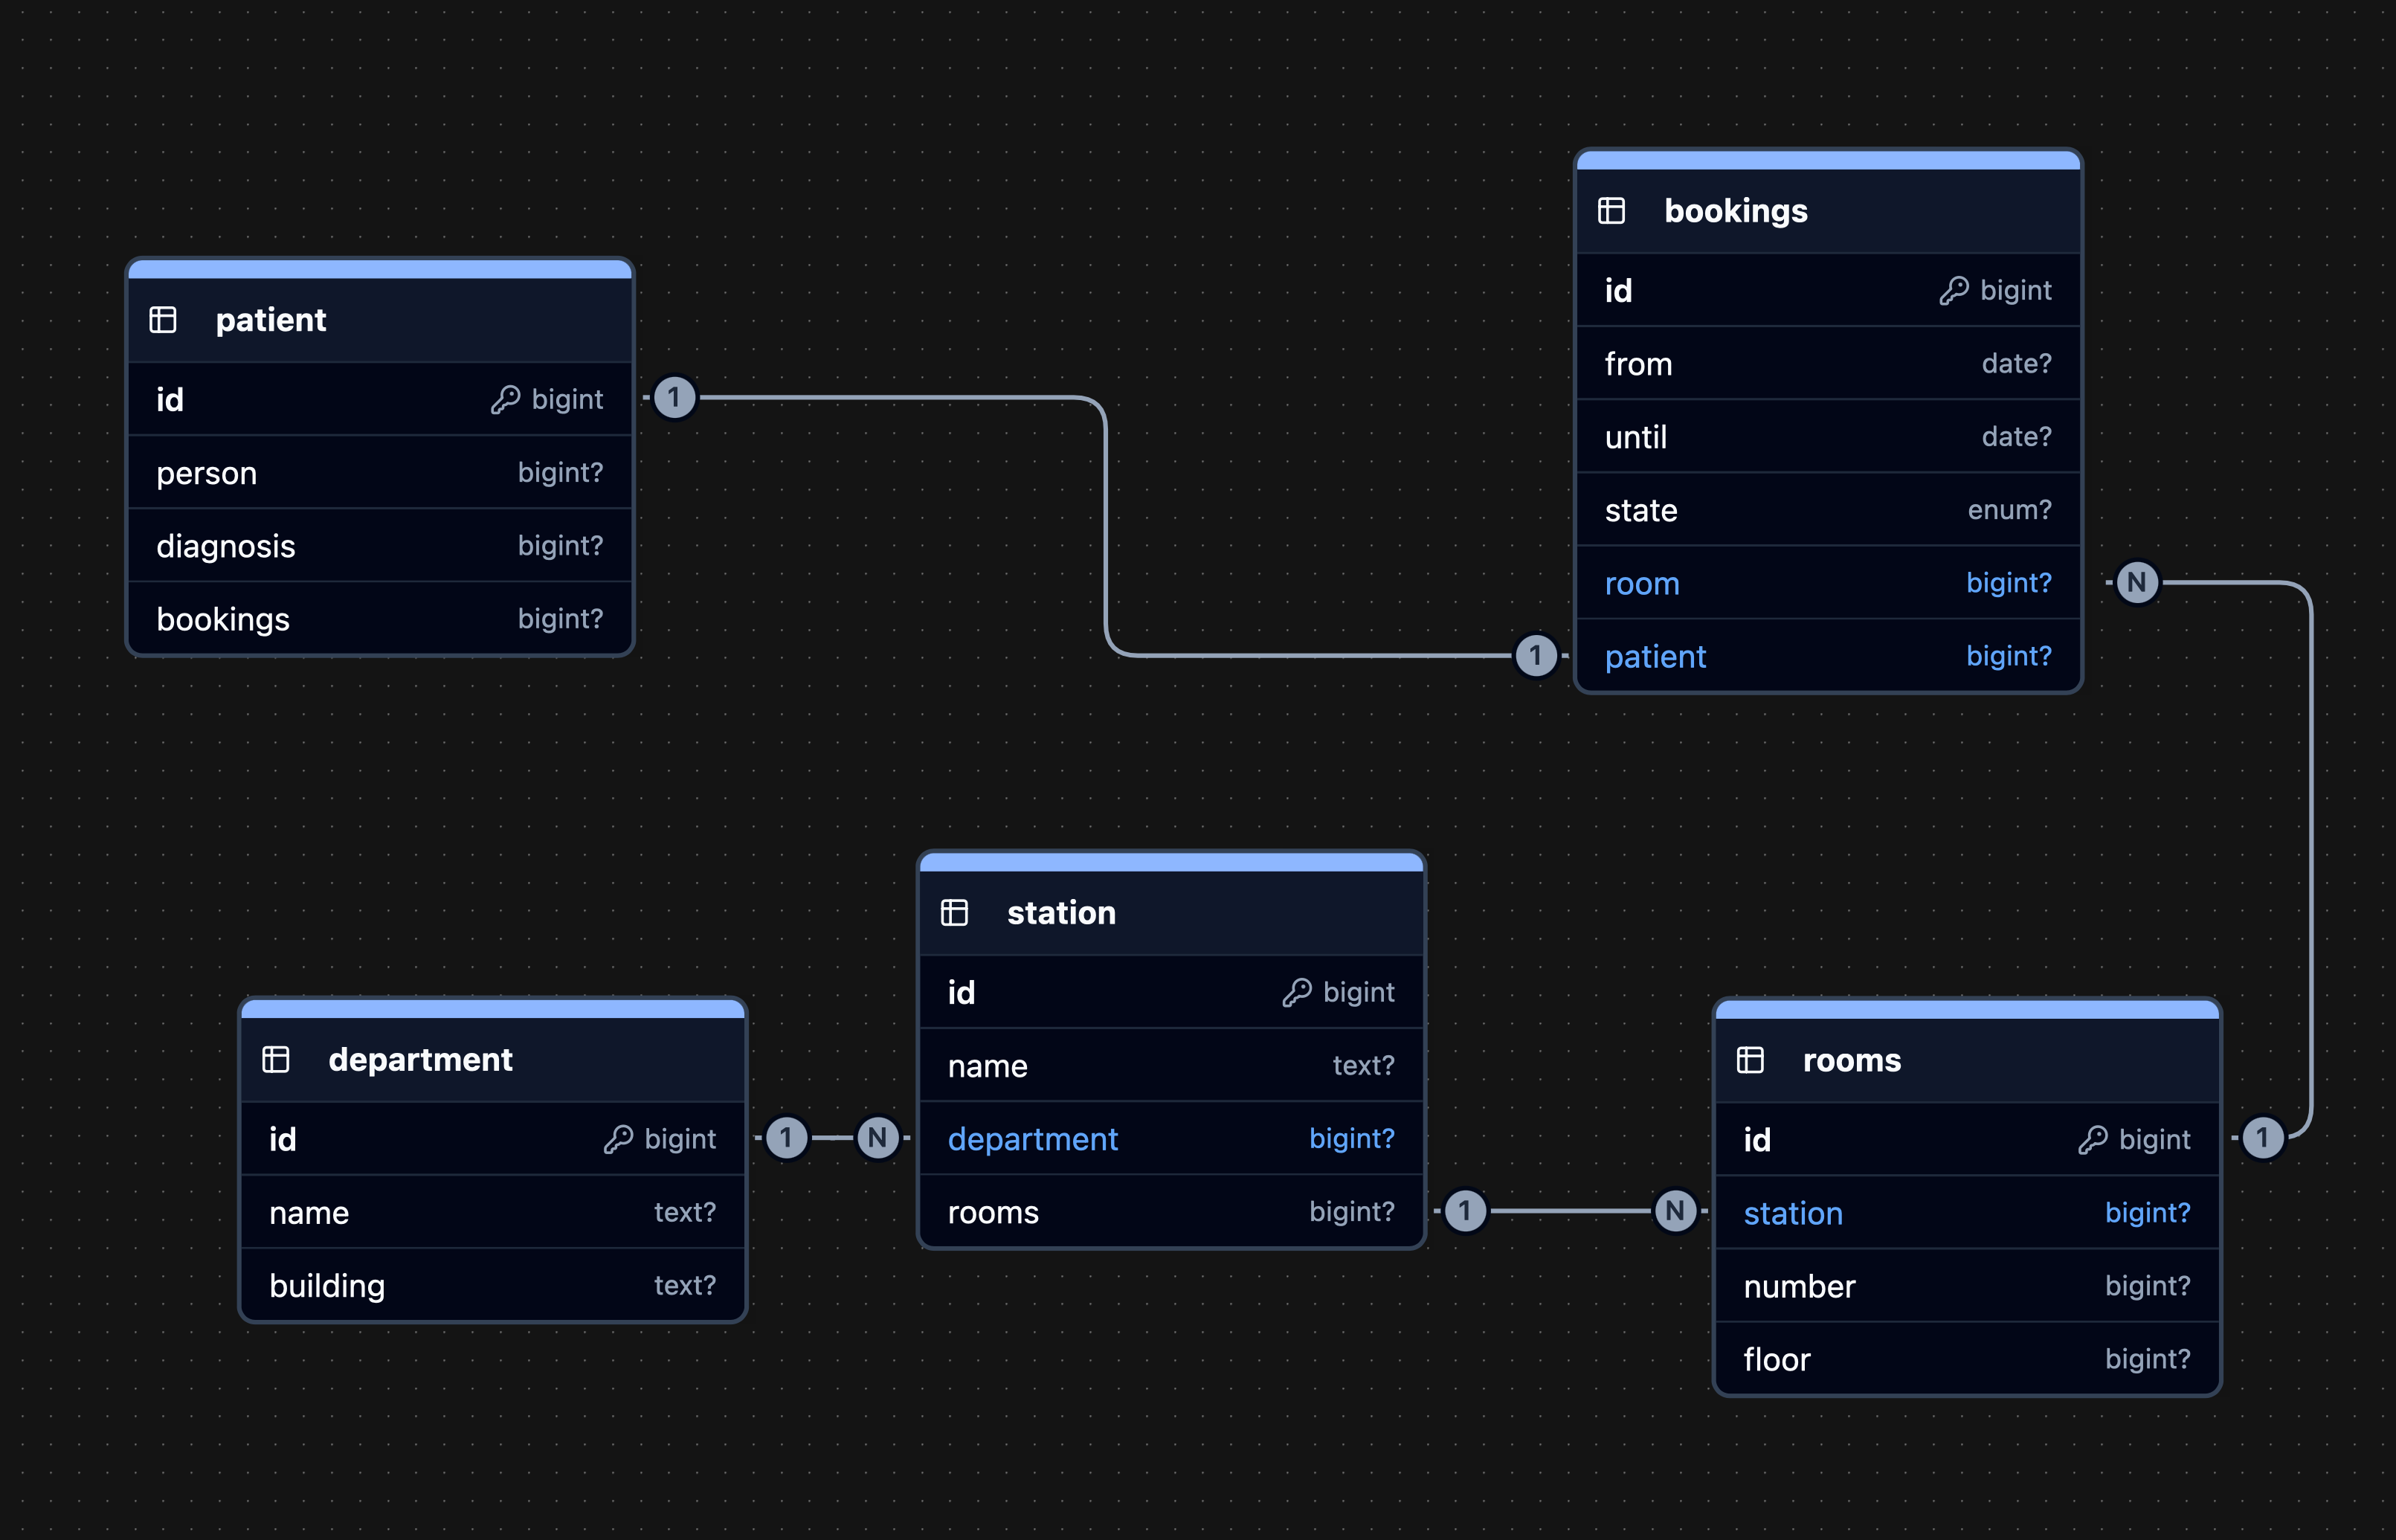
\includegraphics[width=\textwidth]{Bereiche_Datenmodell/Entities_Patients_and_Rooms.png}
    \caption{Resultierende Klassen zur Patienten- und Raumverwaltung}
    \label{fig:patientsAndRoomsUseCases}
\end{figure}

